%!TEX root = ../main.tex

 In terms of scope the aim of the method is to produce plausible lighting for Augmented Reality applications, and thus increase the sense of realism of the composed graphics. This does not mean that imagery that would for all practical purposes be indistinguishable from reality will be achieved. As said earlier, the incompatible lighting is only one of the problems with current AR graphics. In order to achieve complete realism all the other problems would have to be tackled as well. The method also does not attempt to improve other aspects of AR, such as tracking. And so the experiment is designed only to evaluate the similarity of a real object and a virtual representation of the same object in the same controlled lighting conditions.\newline
\section{Setup}
In order to test the results a real object with a variety of materials was chosen, in this case it was an Xbox 360 controller with a custom paint job. A 3D model of the same Xbox 360 controller was modified to match the custom paint job and the materials were replicated as closely as posible to the real object using Unity's built-in shaders. In the end 4 main shaders were used, a highly reflective plastic for the borders and some of the buttons, a more matte plastic for the main body, a completely specular chrome for the Xbox button and a semi-transparent and glossy plastic for the colored buttons. The choice of this motif was based both on the ease to find a reliable 3D counterpart for a real object and on the already wide variety of materials present in the object.\newline
In order to provide a ground truth for a reliable size by side comparison a screen capture of the application running while both the real and virtual object are in the frame, in similar positions and orientations and affected by controlled lighting that is also simulated using the method for the virtual counterpart.\newline
As for benchmarking how this method stands in comparison to other similar ones, the conditions of the experiments presented in the results section for the methods in \cite{kanbara2004}, \cite{karsh2014} and \cite{pessoa2011} are replicated in terms of similar setting and virtual objects used. The resulting images are compared to the ones from their methods.\newline
The actual way in which the experiment is conducted is defined in the following scenario:
\begin{itemize}
    \item \textbf{Setting:} A room with consistent and invariable lighting is used and some kind of flat surface to lay the objects on. An Xbox 360 controller with the characteristics described previously and a marker to track the virtual object.
    \item \textbf{Requirements:} A mobile device running the developed demo application, a marker for virtual objects. A real object and its corresponding virtual counterpart, modelled as close as possible. 
    \item \textbf{Goals:} Obtaining a set of images that will enable readers and experimenters alike to make a fair comparison of the method application, side by side with a real object counterpart.
    \item \textbf{Actions:} Place the real object on top of the marker and take a picture with the same device running the demo application. Then remove the object and take screen captures of the augmented scene using a commercial solution and subsequently the method demo application.
     \item \textbf{Benchmark:} The image result yielded by the method, as well as the  time per frame will be captured and used for comparison's sake and benchmarking head to head with the results from similar methods.
\end{itemize}

\section{Results}

\begin{figure}[H]
    \centering
    \begin{minipage}{0.45\textwidth}
        \centering
        \includegraphics[width=0.95\textwidth]{Figures/res1.JPG} % first figure itself
        \caption{Side by side comparison of the real and virtual object}
    \end{minipage}\hfill
    \begin{minipage}{0.45\textwidth}
        \centering
        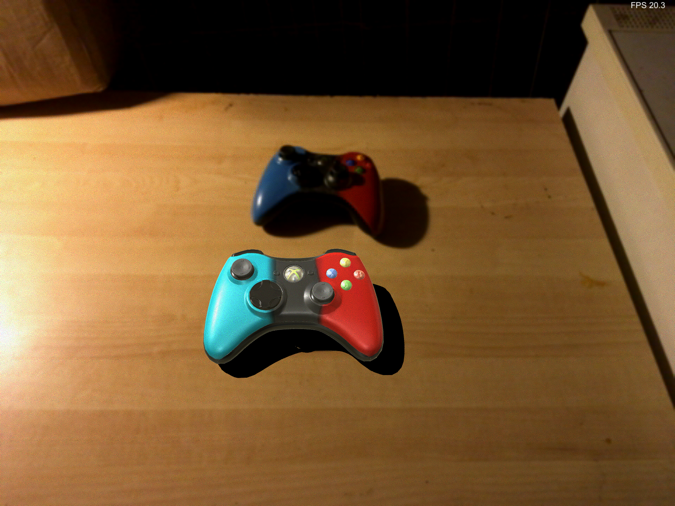
\includegraphics[width=0.95\textwidth]{Figures/rest5.JPG} % second figure itself
        \caption{Side by side comparison of the real and virtual object on a different setting}
    \end{minipage}
\end{figure}

\begin{figure}[H]
    \centering
    \begin{minipage}{0.45\textwidth}
        \centering
        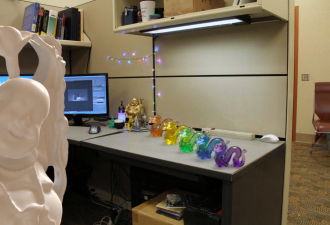
\includegraphics[width=0.95\textwidth]{Figures/budaDragonKarsch.jpg} % first figure itself
        \caption{Karsch's method results}
    \end{minipage}\hfill
    \begin{minipage}{0.45\textwidth}
        \centering
        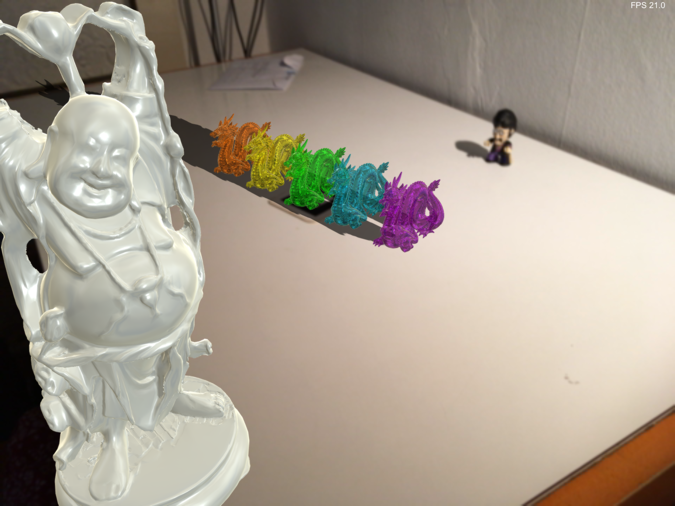
\includegraphics[width=0.95\textwidth]{Figures/budaDragon.JPG} % second figure itself
        \caption{This methods's results}
    \end{minipage}
\end{figure}

\begin{figure}[H]
    \centering
    \begin{minipage}{0.45\textwidth}
        \centering
        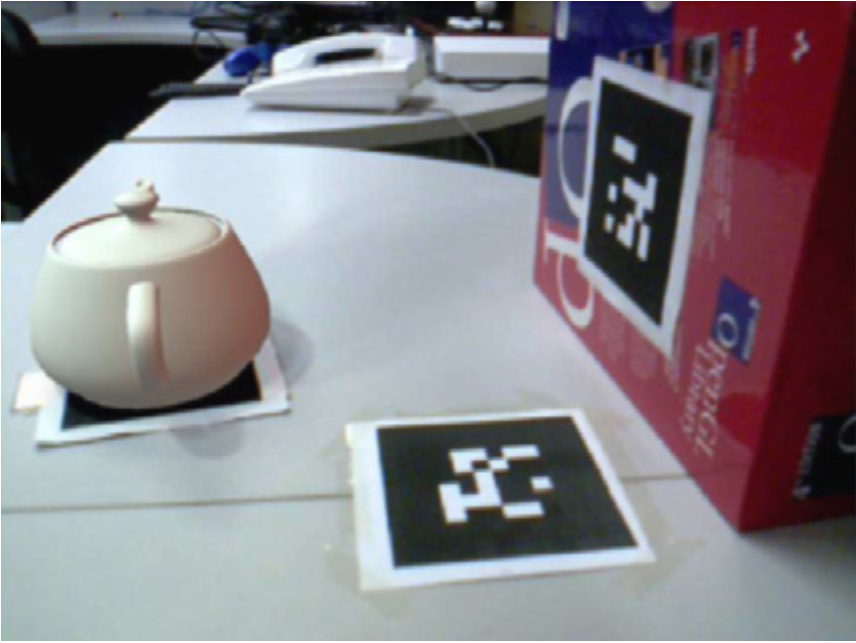
\includegraphics[width=0.95\textwidth]{Figures/Pessoa.png} % first figure itself
        \caption{Pessoa's method results}
    \end{minipage}\hfill
    \begin{minipage}{0.45\textwidth}
        \centering
        \includegraphics[width=0.95\textwidth]{Figures/kanbara.jpg} % first figure itself
        \caption{Kanbara's method results}
    \end{minipage}\hfill
    \begin{minipage}{0.45\textwidth}
        \centering
        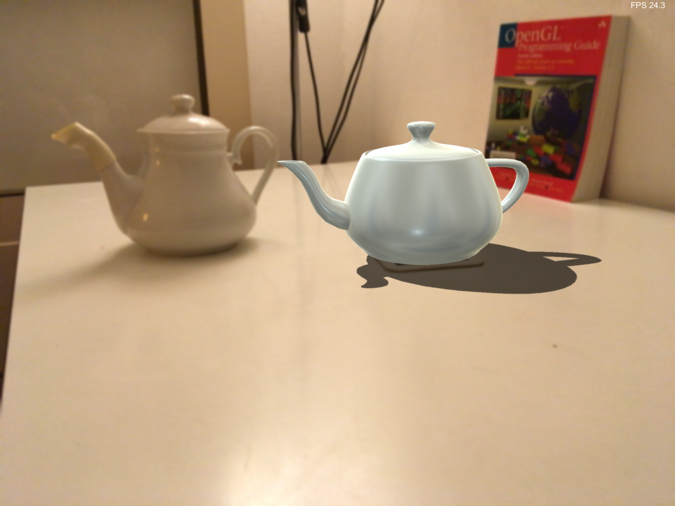
\includegraphics[width=0.95\textwidth]{Figures/teapot1.JPG} % first figure itself
        \caption{This method's method results}
    \end{minipage}\hfill
    \begin{minipage}{0.45\textwidth}
        \centering
        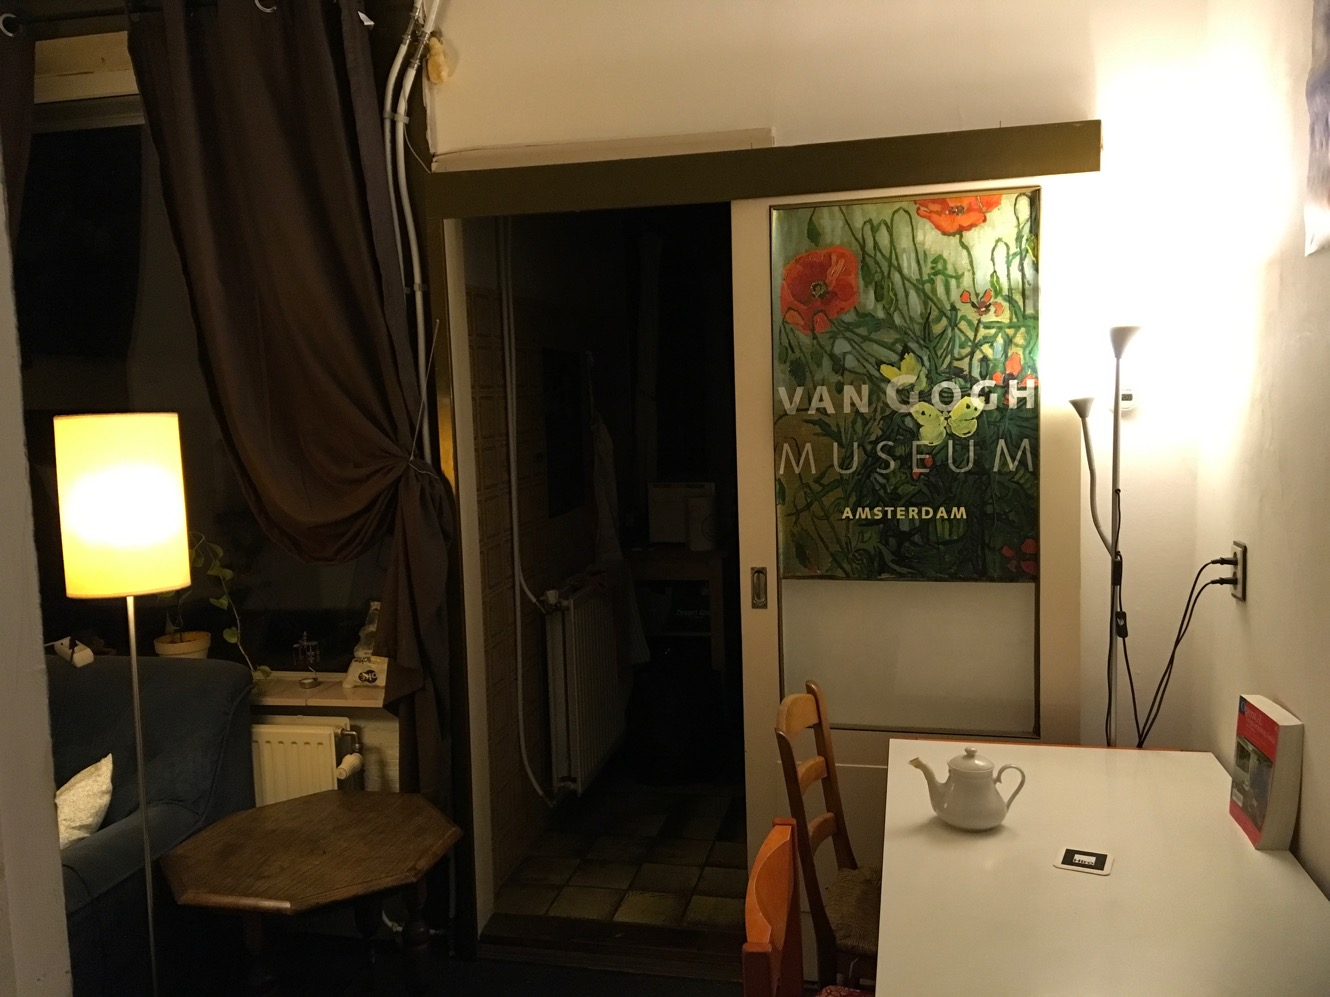
\includegraphics[width=0.95\textwidth]{Figures/setting.JPG} % second figure itself
        \caption{This methods's setting}
    \end{minipage}
\end{figure}